\documentclass[parskip=half,
 fontsize=12pt, bibtotoc,
 ngerman]
 {article}
%%Präambel
\usepackage[utf8]{inputenc} 
\usepackage[ngerman]{babel}
\usepackage{libertine}
\usepackage[T1]{fontenc}
%\usepackage{geometry}
\usepackage[bottom]{footmisc}
\usepackage{setspace}
\usepackage{anysize}
%Bibliographie
\usepackage{typearea}
\usepackage{biblatex}
\usepackage{amssymb}
\usepackage{amsmath}
\usepackage{algorithm}
\usepackage{algorithmic}
\usepackage{graphicx}
\renewcommand{\postnotedelim}{\addcolon\addspace}
%\usepackage[babel,german=guillemets]{csquotes}
\DeclareFieldFormat{postnote}{#1}
\bibliography{abschlussbericht}
\author{Terese Haimberger, Lea Helmers, Mahmoud Kassem, Daniel Theus, Moritz Walter}
\title{Softwareprojekt: Rekonstruktion metrischer Graphen}
\date{}
\usepackage[left=3cm,right=4cm,top=2cm,bottom=2cm]{geometry}
\usepackage{hyperref}
\setlength{\parindent}{0pt}

\begin{document}
\maketitle
\tableofcontents
\newpage
\onehalfspacing
\section{Einleitung}
\subsection{Motivation und Problemstellung}
Im Rahmen des Softwareprojekts "`Anwendungen effizienter Algorithmen"' haben wir uns damit befasst, einen Algorithmus umzusetzen, der aus einer Punktmenge den zugrundeliegenden Graphen sowie dessen Metrik rekonstruiert. Dadurch soll Struktur in gro{\ss}e Mengen geometrischer Daten gebracht werden, was deren Analyse und Weiterverarbeitung erleichtert. Zu verarbeitende Daten können Netzwerke im weitesten Sinne sein, wie beispielsweise GPS-Daten, Strom- und Nachrichtennetze oder astrologische Daten. Häufig enthalten diese Daten Rauschen oder Ausreißer und sind zudem im Allgemeinen sehr umfangreich. Ziel des Algorithmus ist es, die Datenmenge kompakt durch ihre wichtigsten Verzweigungen darzustellen, wodurch sie auf ihre wichtigen Aspekte reduziert wird. So kann eine einfachere Visualisierung und die weitere Analyse und Verarbeitung der Daten ermöglicht werden.
\subsection{Der Algorithmus}
Als Grundlage für unsere Arbeit diente uns ein Paper \cite{chenEa2012}, welches einen Algorithmus für die Rekonstruktion metrischer Graphen beschreibt und dessen Richtigkeit beweist. Die Eingabe besteht dabei aus einem metrischen Raum $\left(Y, d_y\right)$, der aus den Rohdaten konstruiert wird und dem ein metrischer Graph $\left(X, d_x\right)$ zugrunde liegt, den es zu rekonstruieren gilt. Ziel des Algorithmus ist es, diesen zugrunde liegenden Graphen durch einen metrischen Graphen $(\hat{X}, d_{\hat{x}})$ anzunähern und dabei weitestgehend die Abstände von $\left(X, d_x\right)$ in $(\hat{X}, d_{\hat{x}})$ beizubehalten. Zusätzlich zu $\left(Y, d_y\right)$ wird auch ein Parameter $r$ übergeben, der in einigen Schritten des Algorithmus eine wichtige Rolle spielt. Die Erstellung des Graphen $(\hat{X}, d_{\hat{x}})$ wird nun wie folgt durchgeführt:\newline

\begin{enumerate}
\item \textbf{Kanten- und Knotenpunkte bestimmen}\newline
Zunächst wird festgestellt, welche der in $\left(Y, d_y\right)$ enthaltenen Punkte in $(\hat{X}, d_{\hat{x}})$ zu einer Kante und welche zu einem Knoten gehören werden. Dafür wird um alle im Eingabegraphen enthaltenen Punkte ein Kreisring gelegt, wobei der innere Kreis des Kreisrings den Radius $r$ und der äu"sere den Radius ${5\over 3}r$ hat. Für die Punktmenge in diesem Kreisring wird anschlie"send der Rips-Vietoris-Graph mit dem Parameter ${4 \over 3}r$ erstellt. Das bedeutet, dass alle Punkte, die nicht mehr als ${4 \over 3}r$ voneinander entfernt sind, zu einer Zusammenhangskomponente gefasst werden. Daraufhin wird der Grad des jeweiligen Knoten bestimmt, indem die Zusammenhangskomponenten des Rips-Vietoris-Graphen gezählt werden. Enthält der Kreisring um einen Knoten zwei Zusammenhangskomponenten, hat er Grad zwei und es handelt sich um einen Punkt, der im rekonstruierten Graphen $(\hat{X}, d_{\hat{x}})$ zu einer Kante gehören wird. Daher erhält er das Label \textit{edge point}. Ist der Grad ungleich zwei, wird der Punkt zu einem Knoten gehören und wird daher als \textit{preliminary branch point} gekennzeichnet.
Diese Markierung erhalten diese Punkte lediglich vorläufig (\textit{preliminary}), da im Anschluss alle Punkte innerhalb eines Abstands von $2r$ von einem \textit{preliminary branch point} als \textit{branch point} gekennzeichnet werden. Hierbei werden auch die \textit{preliminary branch points} zu \textit{branch points}, womit sich die Punkte in $\left(Y, d_y\right)$ nun in zwei Teilmengen $\mathbb{E}$ und $\mathbb{V}$ aufteilen lassen. In $\mathbb{E}$ sind dabei die \textit{edge points} enthalten und in $\mathbb{V}$ die \textit{branch points}. Der Vorgang wird mit Pseudocode in Algorithm \ref{algo1} veranschaulicht. \newline
\begin{algorithm}
\caption{Kanten- und Knotenpunkte bestimmen}\label{algo1}
\begin{algorithmic}
\FORALL{$y \in Y$} 
\STATE $R \leftarrow C_{{5\over 3}r} \setminus C_r$ 
\STATE $deg\left(y\right) \leftarrow$ \# Zusammenhangskomponenten im Rips-Vietoris-Graphen$_{{4 \over 3}r}\left(R\right)$
	\IF{$deg(y) == 2$}
		\STATE y erhält das Label edge point
	\ELSE 
		\STATE y erhält das Label branch point
	\ENDIF
\ENDFOR
\FORALL{$y \in Y$}
	\IF{$y$ ist nicht weiter als $2r$ von einem preliminary branch point entfernt}
		\STATE y erhält das Label branch point
	\ENDIF
\ENDFOR
\end{algorithmic}
\end{algorithm}
\item \textbf{Struktur des Graphen rekonstruieren}\newline
Anschlie{\ss}end wird für die beiden Mengen $\mathbb{V}$ und $\mathbb{E}$ der Rips-Vietoris-Graph mit dem Parameter $2r$ erstellt. Die dabei entstehenden Zusammenhangskomponenten in $\mathbb{E}$ entsprechen nun den Kanten und jene in $\mathbb{V}$ den Knoten im Graphen $(\hat{X}, d_{\hat{x}})$. Um dessen Struktur zu vervollständigen müssen lediglich noch die Verbindungen zwischen Kanten und Knoten rekonstruiert werden. Dies geschieht, indem zwei Knoten aus  $\mathbb{V}$ genau dann durch eine Kante $e \in \mathbb{E}$ verbunden werden, wenn sie in ihrer Zusammenhangskomponente Punkte haben, die zu Punkten der Zusammenhangskomponente von $e$ einen kleineren Abstand als $2r$ haben.

\item \textbf{Metrik rekonstruieren}\newline
Schlussendlich müssen noch die Längen der Kanten bestimmt werden. Dafür wird jeder Kante in $\hat{X}$ als Länge der Durchmesser ihrer Zusammenhangskomponente, also der längste kürzeste Weg darin, zuzüglich $4r$ zugewiesen.
\end{enumerate} 


\section{Organisation}
\subsection{Programmiersprache}
Da allen Studenten im Team die objektorientierte Programmiersprache Java geläufig war und sie uns als durchaus geeignet für die Aufgabe schien, haben wir uns entschlossen, unser Programm darin zu schreiben.

\subsection{Gruppenaufteilung}
Für das Arbeiten an unserer Software haben wir uns in drei verschiedene Gruppen aufgeteilt. Die eine Gruppe hat sich mit der Vorverarbeitung der Rohdaten beschäftigt, im Wesentlichen also aus den Rohdaten den metrische Raum $\left(Y, d_y\right)$ für die Eingabe des Algorithmus konstruiert. Dabei beschlossen wir, uns auf die Visualisierung von GPS-Daten und Schwarz-Wei"sbildern zu beschr\"anken, sodass es vorrangig darum ging, diese beiden Datengrundlagen so aufzubereiten, dass die nächste Gruppe damit weiterarbeiten konnte. Die zweite Gruppe hat sich mit der Implementierung des Algorithmus, genauer der Rekonstruktion von $(\hat{X}, d_{\hat{x}})$, in Java auseinandergesetzt, während die dritte für die Visualisierung des Graphen $(\hat{X}, d_{\hat{x}})$ zuständig war.

\subsection{Kommunikation}
Damit wir stets alle über die Arbeit unserer Teammitglieder informiert waren, haben wir unsere Ergebnisse auf der Hosting-Plattform \textit{GitHub}\footnote{\url{github.com}} gespeichert und aktualisiert. Um anstehende Aufgaben für alle zugänglich zu dokumentieren haben wir zusätzlich die für Projektmanagement bestimmte Anwendung \textit{Trello} \footnote{\url{trello.com}} genutzt, bei der man ein virtuelles Notizbrett erstellen kann. Hier konnte jeder neue Aufgaben an eine virtuelle Pinnwand hängen und sich dafür als Bearbeiter eintragen. Zusätzlich konnten wir dort den Stand der Arbeit an diesen Aufgaben dokumentieren, wodurch stets jeder darüber informiert war, woran die anderen gerade arbeiteten.

Darüber hinaus haben wir per E-Mail kommuniziert und uns einmal pro Woche in der Universität getroffen, um die wichtigsten Ergebnisse der vergangenen und die Vorhaben für die kommende Woche zu besprechen und festzulegen.
 
\section{Arbeit in den einzelnen Gruppen}
Im Folgenden soll nun ein Überblick darüber gegeben werden, wie die drei verschiedenen Gruppen gearbeitet haben. Die Gruppe, die sich mit der Vorverarbeitung beschäftigt hat, bestand aus zwei Studierenden, jene, die für die Graphenrekonstruktion verantwortlich war, aus drei und für die Visualisierung des rekonstruierten Graphen war ein Student verantwortlich.

\subsection{Preprocessing}
Die Kernaufgabe dieser Gruppe bestand in der Erfassung, sowie der Vorverarbeitung der Eingabedaten in eine für den Algorithmus passende Form.

Als Eingabe sind Schwarz-Weiß-Bilder, sowie GPS-Trace-Route-Dateien gedacht. Aus diesen müssen die Koordinaten der einzelnen Punkte extrahiert werden. Im Falle der GPS-Dateien wurde dazu ein Filter erstellt, welcher die angegebene Datei durchsucht und die Koordinaten (Längen- und Breitengrade) extrahiert. Sollte ein Bild angegeben werden, wird jeder Bildpunkt geprüft, wobei von jedem schwarzen die Pixelkoordinaten erfasst werden.

Da eventuell eine sehr große Punktmenge das Resultat sein kann, gibt es die Möglichkeit zur Reduzierung in Form der EpsilonNet-Klasse, welche durch Angabe eines Parameters (\emph{epsilon}) redundante Punkte entfernt. Dabei wird ein Algorithmus verwendet, der unter Verwendung eines Gitters ein metrisches Epsilon-Netz in linearer Zeit berechnet.\footnote{Sariel Har-Peled und Benjamin Raichel. Net and Prune: A Linear Time Algorithm for Euclidean Distance Problems. \url{http://web.engr.illinois.edu/~raichel2/aggregate.pdf}, 8. November 2012. (Beweis zum Lemma 2.2)}

Die Punkte werden in einem Set platziert und sind so zur weiteren Verarbeitung zugänglich.

Anschließend ist es das Ziel, diese Punkte in einen metrischen Raum (\textit{metric space}) umzuformen, d.\,h. die Punktmenge so zu strukturieren, dass wir möglichst schnell und einfach die paarweisen Abstände zwischen den Punkten berechnen können.

Dazu wird zuerst die Delaunay-Triangulierung der Punktmenge berechnet (mithilfe der DelaunayTriangulationBuilder-Klasse der JTS Topology Suite). Anhand dieser Triangulierung wird ein Nachbarschaftsgraph erstellt. Der Graph besteht aus allen Knoten der Triangulierung und allen Kanten, deren Radius einen bestimmten Wert (\emph{alpha}) nicht überschreitet. (Der einzige Unterschied zum Alpha-Komplex ist, dass der Nachbarschaftsgraph keine Dreiecke enthält.) Als Datenstruktur werden dabei Adjazenzlisten verwendet.

Die Berechnung der Abstände erfolgt dann mithilfe des Floyd-Warshall-Algorithmus zur Bestimmung des kürzesten Pfades. Da diese Berechnung lange dauert, berechnen wir alle Abstände einmal und speichern sie in einer zweidimensionalen Tabelle (realisiert durch verschachtelte HashMap-Objekte). Bei der Rekonstruktion des Graphen können wir dann einfach auf die schon berechneten Abstände zugreifen.

Nun liegen alle benötigten Daten für den eigentlichen Algorithmus vor und werden in Form eines MetricSpace-Objektes übergeben.

\begin{figure}[h]
\centering
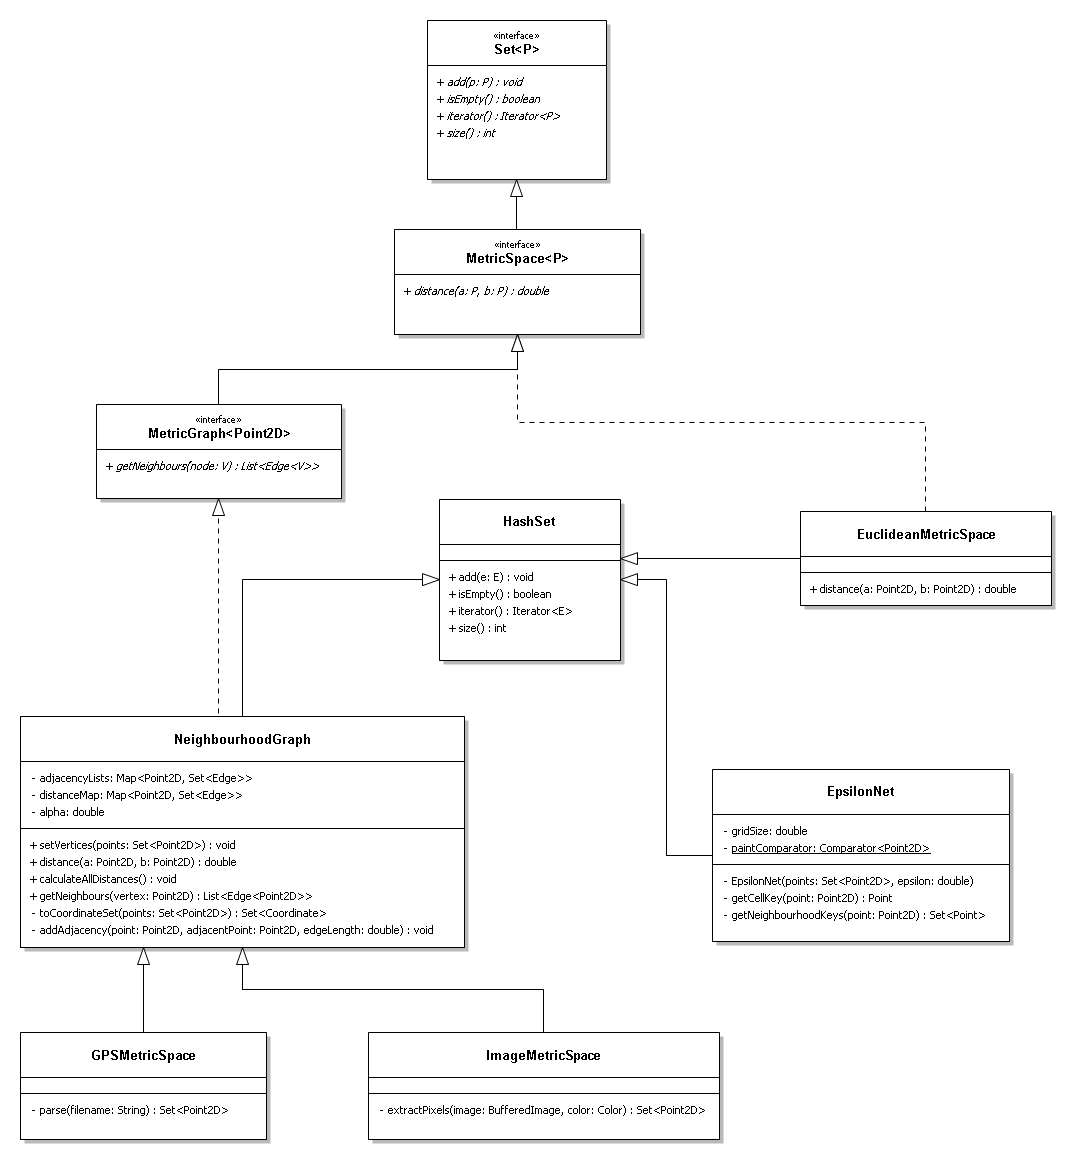
\includegraphics[scale=0.5]{preprocessing.png}
\end{figure}

\subsection{Rekonstruktion}

\begin{figure}[h]
\centering
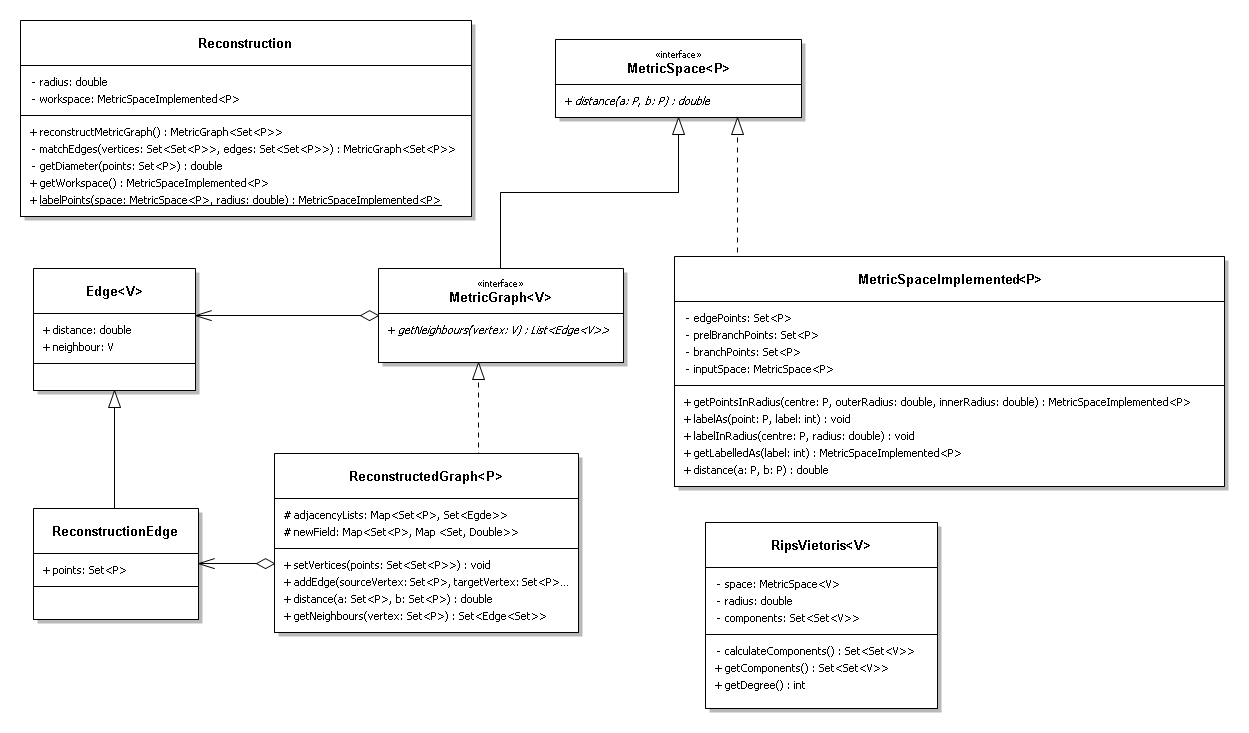
\includegraphics[scale=0.5]{main.png}
\end{figure}

\subsection{Visualisierung}

\section{Testen}

\section{Schwierigkeiten und Verbesserungsvorschläge}

Eine grundsätzliche Schwierigkeit war das Testen fertiger Module.
Aufgrund der Datenfluss-ähnlichen Struktur des Gesamtprogramms kann
ein kleiner Fehler in der Vorverarbeitung massiven Einfluss
auf das Endergebnis nehmen. Da dieses Ergebnis graphischer Natur ist,
war wirkliches Testen aber erst nach Erstellung einer graphischen Ausgabe
(Prototyp) möglich. Im Falle des Epsilon-Netz ließ sich so beispielsweise 
zuverlässiges Aussortieren von nicht benötigten Punkten erst spät testen,
da anhand der blanken Koordinaten die Auswirkungen sich nicht gut genug
erkennen ließen und die Menge als ganzes nur schwer zu erfassen war.

Ideen für weitere Features bzw. Änderungen an Algorithmen gab es einige, 
allerdings machte der Zeitmangel die Umsetzung zu Nichte. So waren
als Verbesserungen z.\,B. eine Einbeziehung des Zeitstempels von GPS Daten
zur Verbesserung des Nachbarschaftsgraphen, die Abstandsberechnung mithilfe des
Algorithmus von Dijkstra statt Floyd-Warshall um die Laufzeit zu senken,
eine automatisierte Möglichkeit zur optimalen Bestimmung der Parameter oder
auch die Berechnung von Orthodromen um den Abstand in km anzugeben, angedacht.

\section{Zusammenfassung}
\printbibliography

\end{document}